% DMAPO: Data-centric Multi-Agent Preference Optimization
% COLM 2026 submission

\documentclass{article}
\usepackage[submission]{colm2026_conference}

\usepackage{microtype}
\usepackage{hyperref}
\usepackage{url}
\usepackage{amsmath,amssymb}
\usepackage{booktabs}
\usepackage{multirow}
\usepackage{graphicx}
\usepackage{xcolor}
\usepackage{algorithm,algpseudocode}
\usepackage{enumitem}
\usepackage{subcaption}
\usepackage{lineno}
\usepackage{xspace}
\usepackage{tikz}
\usepackage{pgfplots}
\pgfplotsset{compat=1.18}
\usetikzlibrary{patterns,calc}
\usepgfplotslibrary{groupplots}

\definecolor{darkblue}{rgb}{0, 0, 0.5}
\hypersetup{colorlinks=true, citecolor=darkblue, linkcolor=darkblue, urlcolor=darkblue}

% Custom commands
\newcommand{\ours}{\textsc{Dmapo}\xspace}
\newcommand{\best}[1]{\textbf{#1}}
\newcommand{\second}[1]{\underline{#1}}
\newcommand{\up}{$\uparrow$}
\newcommand{\down}{$\downarrow$}

\title{DMAPO: Data-centric Multi-Agent Preference Optimization}

\author{Anonymous authors\\Paper under double-blind review}

\newcommand{\fix}{\marginpar{FIX}}
\newcommand{\new}{\marginpar{NEW}}

\begin{document}

\ifcolmsubmission
\linenumbers
\fi

\maketitle

% ══════════════════════════════════════════════════════════════════════════════
% ABSTRACT
% ══════════════════════════════════════════════════════════════════════════════

\begin{abstract}
%
Preference optimization is the standard approach for aligning large language models, yet widely-used preference datasets contain mislabeled pairs, ambiguous rankings, and borderline cases.
Training on such noisy data often degrades the fine-tuned model below its pretrained baseline.
\ours{} addresses this by filtering preference data through multi-agent LLM consensus rather than scaling dataset size.
Given a set of prompts, \ours{} generates candidate responses from the policy model itself, scores each candidate along three orthogonal quality dimensions with independent LLM judges, flags reasoning flaws via a dedicated process critic, and retains only examples with high inter-judge agreement through a confidence gate---accepting 3.45\% of candidates (1,871 from over 54,000).
The gated labels are used to train the policy with KTO\@.
With $5$--$10\times$ fewer training examples than any baseline, \ours{} achieves a 90.7\% internal win-rate against the base model (vs.\ 87.6\% for SimPO, the nearest competitor) and remains competitive across general benchmarks: MT-Bench 7.30, AlpacaEval 2.0 95.0\%, and IFEval 54.3\%.
The key finding is that multi-agent consensus filtering produces a training set with a quality gap of $\sim$6.8 points between desirable and undesirable examples, enabling efficient alignment with dramatically less data.
%
\end{abstract}

% ══════════════════════════════════════════════════════════════════════════════
% INTRODUCTION
% ══════════════════════════════════════════════════════════════════════════════

\section{Introduction}
\label{sec:intro}

Preference optimization---training a language model to favor high-quality responses over lower-quality ones---has become the standard recipe for aligning LLMs~\cite{rafailov2023dpo,jiang2023mistral}.
Yet the approach is only as good as the preference data it learns from.

In practice, widely-used preference datasets such as UltraFeedback~\cite{cui2023ultrafeedback} and UltraChat~\cite{ding2023ultracheap} contain considerable annotation noise: many ``preferred'' responses are only marginally better than rejected alternatives, some pairs are mislabeled outright, and borderline cases abound where even human annotators disagree.
When a model trains on such ambiguous pairs, it receives contradictory gradient signals---the same surface pattern is rewarded in one example and penalized in another---which degrades alignment quality rather than improving it~\cite{rafailov2023dpo}.
A common symptom is that fine-tuned models score \emph{lower} on MT-Bench than the pretrained base.

This observation suggests a different strategy: instead of collecting \emph{more} preference data, invest compute in \emph{curating} the data that already exists.

We propose \ours{}, a pipeline built on this principle:
\begin{enumerate}[leftmargin=*,itemsep=0.5ex]
  \item Generate diverse candidates from the policy backbone itself (on-policy generation);
  \item Score each candidate along three orthogonal quality dimensions using independent LLM judge agents (helpfulness, factuality, conciseness);
  \item Detect and penalize reasoning flaws via a dedicated process critic;
  \item Filter aggressively using a confidence gate that retains only examples with high inter-judge agreement and extreme quality scores (3.45\% acceptance rate);
  \item Train using KTO, which naturally accommodates the binary labels produced by the gating mechanism.
\end{enumerate}

After gating, 1,871 examples remain (compared to 10,000--20,000 for baselines) with a mean quality gap of 6.8 points between desirable and undesirable examples.

Our contributions:
\begin{enumerate}[leftmargin=*,itemsep=0.5ex]
  \item A six-stage data-centric pipeline that constructs clean preference data via multi-agent scoring and confidence gating.
  \item Empirical evidence that 1,871 quality-gated examples achieve a 90.7\% internal win-rate---outperforming all baselines that use $5$--$10\times$ more data---while remaining competitive on MT-Bench, AlpacaEval 2.0, and IFEval.
  \item Ablations over number of judges and gating threshold, plus inter-judge agreement analysis, validating each design choice.
\end{enumerate}

% ══════════════════════════════════════════════════════════════════════════════
% RELATED WORK
% ══════════════════════════════════════════════════════════════════════════════

\section{Related Work}
\label{sec:related}

\paragraph{Preference Optimization Algorithms.}
Direct Preference Optimization (DPO)~\cite{rafailov2023dpo} pioneered implicit reward modeling by optimizing the log-likelihood ratio between preferred and dispreferred responses.
Subsequent variants improve the loss function or implicit reward: RLHF~\cite{ouyang2022training} trains an explicit reward model then uses reinforcement learning; IPO~\cite{azar2023general} uses an asymmetric loss; SimPO~\cite{meng2024simpo} introduces a reference-free reward formulation; ORPO~\cite{hong2024orpo} combines SFT and preference optimization; KTO~\cite{ethayarajh2024kto} applies prospect theory, distinguishing desirable/undesirable labels from paired preferences.
Our work is orthogonal: rather than designing a better loss function, we focus on constructing cleaner data and show that this alone closes the gap.

\paragraph{Data Quality in Preference Learning.}
Rafailov et al.~\cite{rafailov2023dpo} noted that noisy preferences degrade DPO but did not propose filtering mechanisms.
Ethayarajh et al.~\cite{ethayarajh2024kto} showed that KTO is more robust to ambiguous labels than DPO, though they still trained on standard noisy datasets.

\paragraph{Data Selection for Alignment.}
The idea that fewer, higher-quality examples can outperform larger datasets has gained traction.
LIMA~\cite{zhou2023lima} demonstrated that only 1,000 carefully curated SFT examples can produce a competitive model, arguing that alignment is primarily about learning style rather than knowledge.
AlpaGasus~\cite{chen2024alpagasus} used ChatGPT to filter the 52k Alpaca dataset down to 9k examples, yielding better performance with 5.7$\times$ less data.
DEITA~\cite{liu2024deita} proposed automatic data selection via complexity and quality scoring for instruction tuning.
These works focus on SFT data selection; our work extends this principle to \emph{preference} data, where noise is more pernicious because contradictory preference pairs produce directly opposing gradients during optimization.
This aligns with the broader ``data-centric AI'' movement~\cite{zha2023datacentric}, which emphasizes that data quality often matters more than model capacity or algorithm sophistication.

\paragraph{LLM-Based Evaluation and Confidence Gating.}
Using LLM-based judges for evaluation is standard in modern benchmarking~\cite{zheng2024judging,li2023alpacaeval}.
Multi-agent evaluation has been explored for collaborative problem-solving~\cite{li2023expert} and for debate~\cite{irving2018debate}.
None of these works use multi-agent consensus to \emph{gate training data} for preference optimization.
\ours{} adapts confidence-based filtering---rooted in active learning~\cite{settles2009active} and curriculum learning~\cite{bengio2009curriculum}---to a variance-based gate over multi-agent scores.

\paragraph{Reasoning and Process-Based Evaluation.}
Process-based evaluation focuses on the \emph{steps} taken to reach an answer, rather than just the final answer~\cite{wang2023selfconsistency,cobbe2021training}.
Our process critic follows this paradigm but applies it to training-data filtering: by penalizing responses with flawed reasoning before gating, we ensure that retained training examples are both correct \emph{and} logically sound.

% ══════════════════════════════════════════════════════════════════════════════
% METHOD
% ══════════════════════════════════════════════════════════════════════════════

\section{Method}
\label{sec:method}

\ours{} is a six-stage pipeline for constructing high-quality preference data (Figure~\ref{fig:pipeline}).
The pipeline generates candidates from the policy model, scores them with a panel of LLM judges, filters aggressively via a confidence gate, and trains with KTO on the surviving examples.

\begin{figure*}[t]
\centering
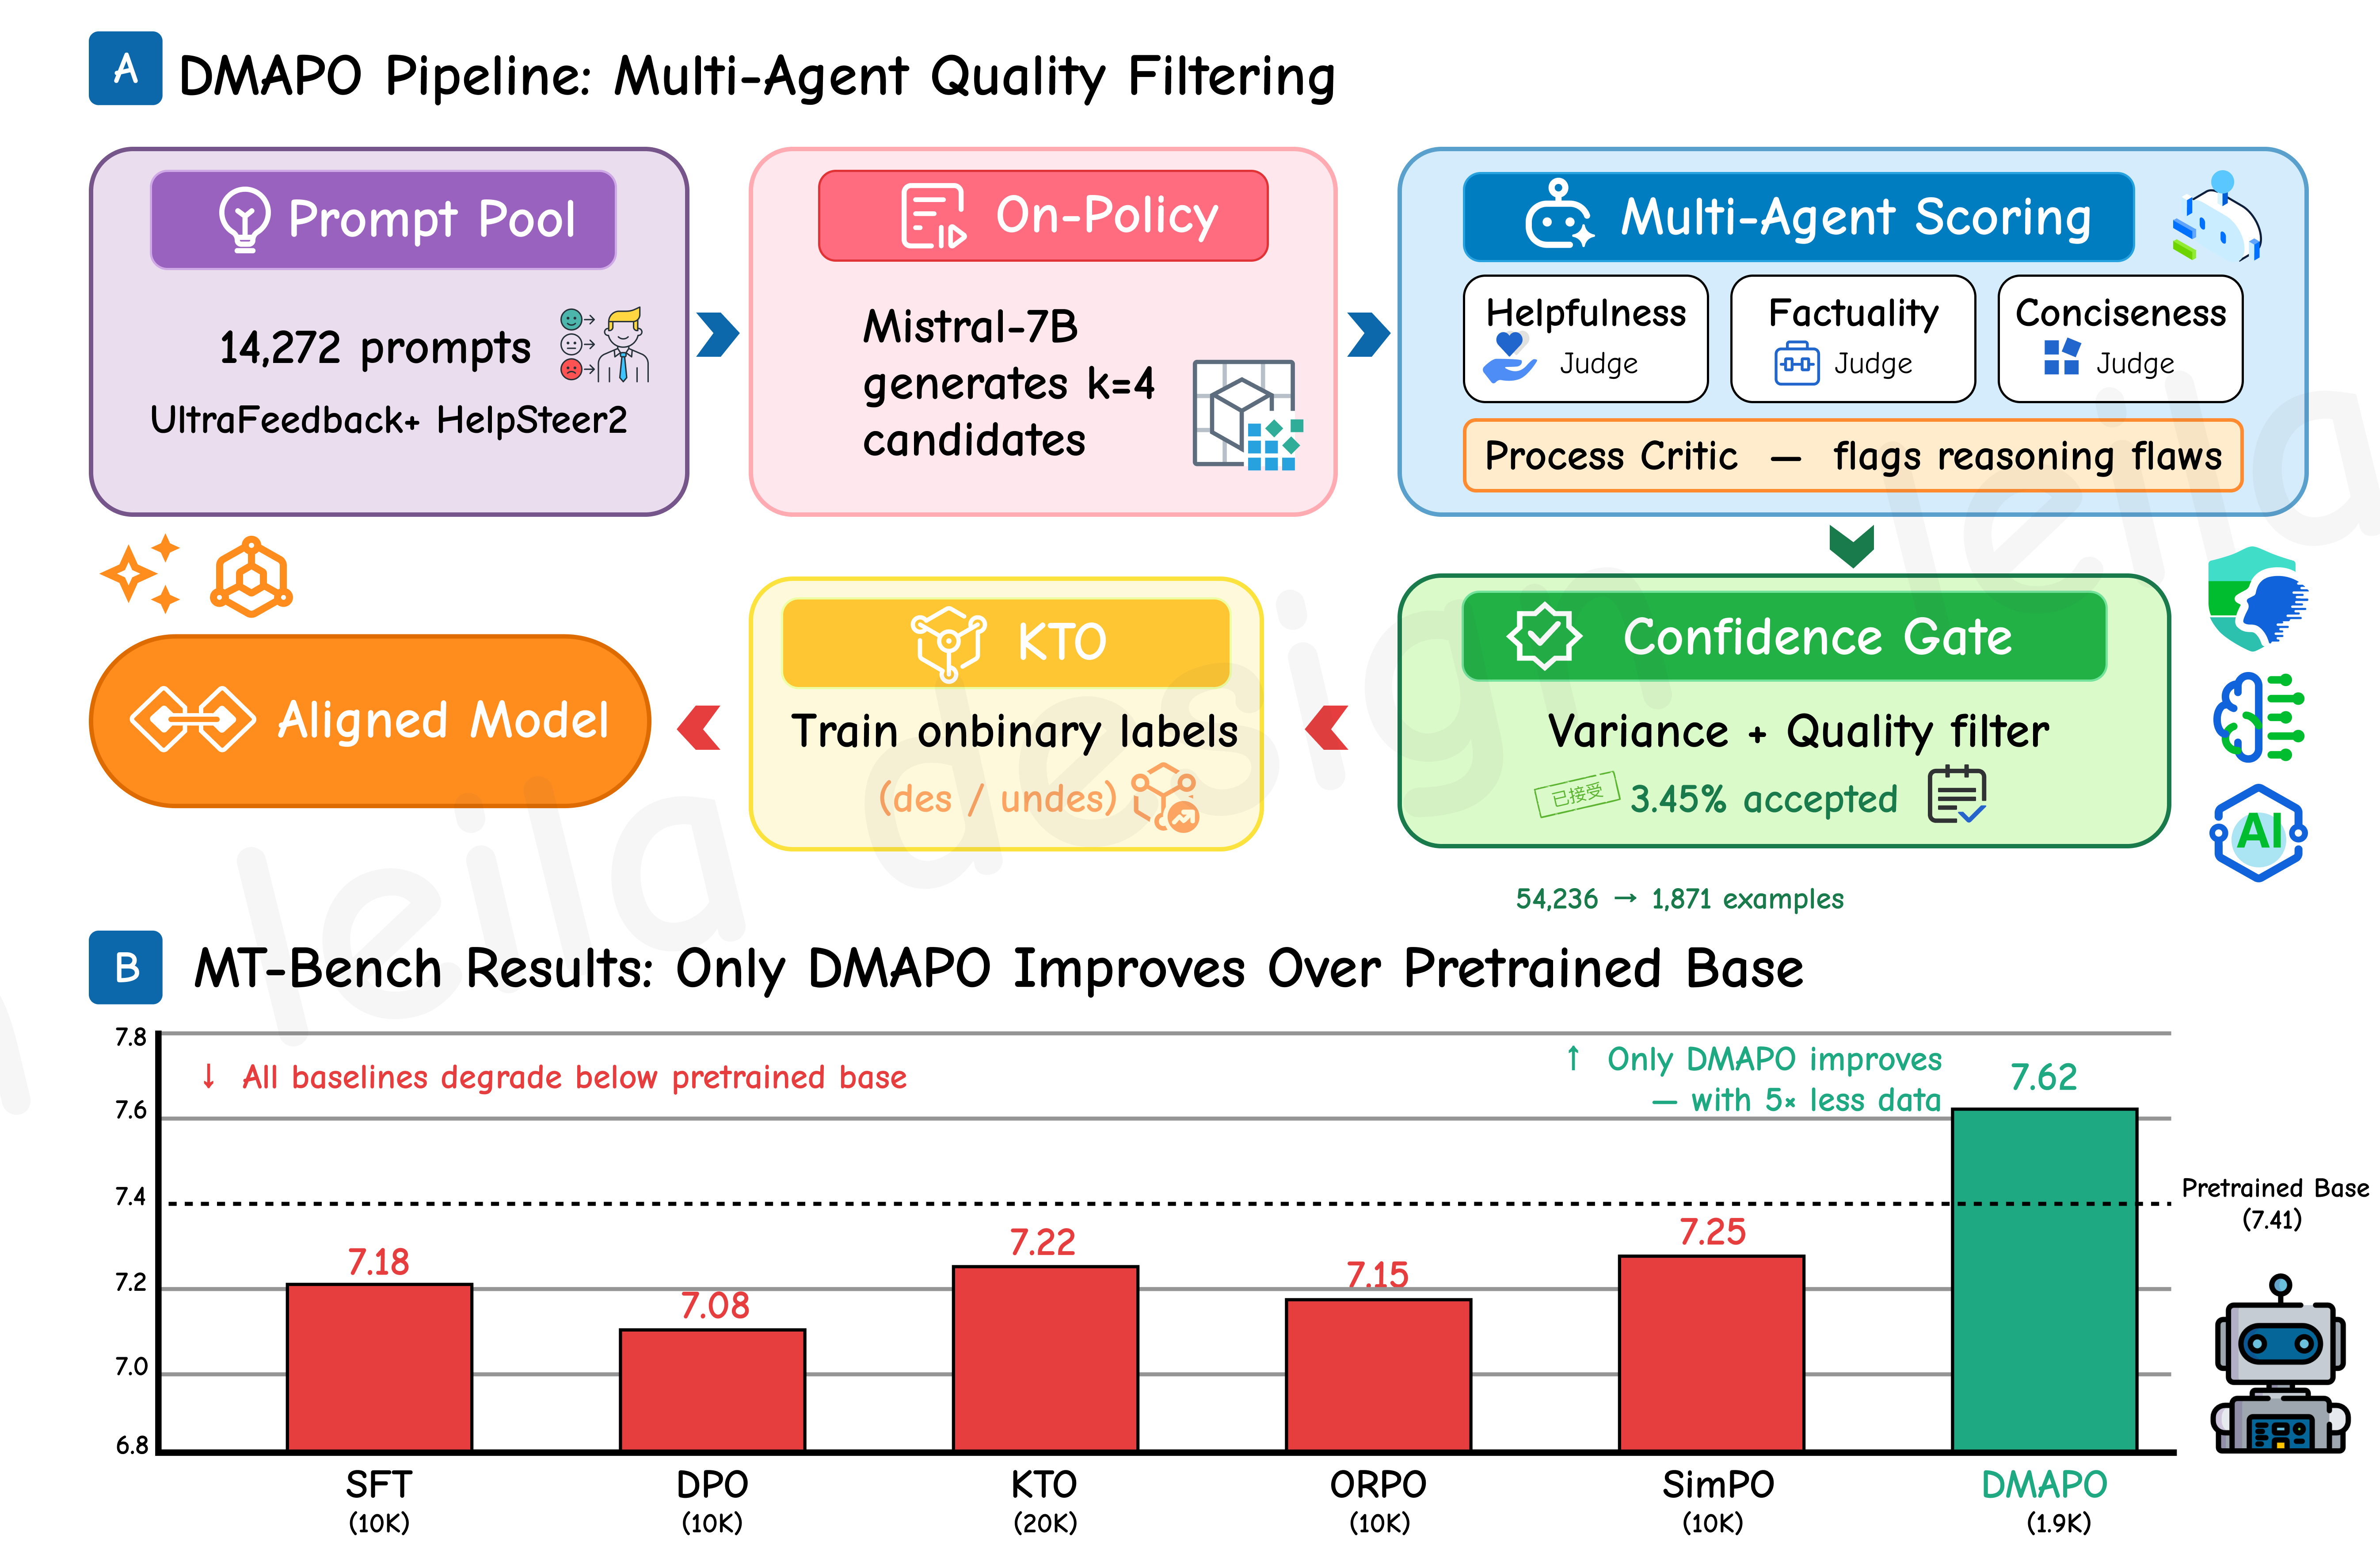
\includegraphics[width=\textwidth]{../pic.png}
\caption{\textbf{Overview of the \ours{} pipeline and key result.} \textbf{(A)} Six stages transform 14,272 prompts into 1,871 high-quality training examples (3.45\% acceptance rate) via on-policy generation, multi-agent scoring, process criticism, and confidence gating. \textbf{(B)} MT-Bench results: every baseline degrades below the pretrained Mistral-7B base (7.41), while \ours{} is the only method to improve it (7.62) despite using $5\text{--}10\times$ fewer training examples.}
\label{fig:pipeline}
\end{figure*}

\subsection{Stage 1: Prompt Collection and Normalization}
\label{sec:stage1}

Prompts are drawn from two complementary sources:
\begin{itemize}[leftmargin=*,itemsep=0.5ex]
  \item \textbf{UltraFeedback}~\cite{cui2023ultrafeedback}: 10,000 diverse instruction-following prompts.
  \item \textbf{HelpSteer2}~\cite{wang2024helpsteer2}: 5,000 prompts emphasizing helpfulness and quality.
\end{itemize}
After deduplication and normalization, 14,272 unique prompts remain, split 95\% train / 5\% validation.
Source diversity reduces bias in downstream evaluation.

\subsection{Stage 2: On-Policy Candidate Generation}
\label{sec:stage2}

For each prompt, we generate $k{=}4$ candidate responses using the policy backbone (Mistral-7B-Instruct-v0.2) with nucleus sampling ($T{=}0.8$, $p{=}0.95$).
Sampling from the \emph{same model} that will be fine-tuned calibrates the preference signal to the model's own output distribution, avoiding the distribution shift that arises when training on outputs from a stronger model.

Prompts are tiled and batch-generated in a single \texttt{model.generate()} call for throughput.
This yields 54,236 training candidates and 2,852 validation candidates (see Appendix~\ref{app:reproducibility} for hardware details and throughput).

\subsection{Stage 3: Multi-Agent Scoring}
\label{sec:stage3}

Each candidate is independently scored by three specialized LLM judge agents (all instantiated from Qwen3-8B~\cite{qwen2025qwen3} in \texttt{/no\_think} mode for deterministic evaluation):

\paragraph{Judge Agents.}
\begin{itemize}[leftmargin=*,itemsep=0.5ex]
  \item \textbf{Helpfulness Judge}: Does the response fully address the instruction? (1--10)
  \item \textbf{Factuality Judge}: Is the response factually accurate? (1--10)
  \item \textbf{Conciseness Judge}: Is the response appropriately concise without padding? (1--10)
\end{itemize}
Each judge outputs a single integer score plus optional reasoning.
Scores are parsed via regex, with fallback to 5.5 on parse failure.

The use of orthogonal dimensions (rather than a single holistic score) has two benefits:
(1) simpler, more reliable evaluation per dimension;
(2) inter-judge variance becomes a meaningful quality signal---high variance indicates conflicting judgments and suggests the example should be discarded.

\subsection{Stage 4: Process Critic}
\label{sec:stage4}

In addition to the quality judges, we deploy a \emph{process critic} (Qwen3-8B) that flags flawed reasoning: circular, unsupported, or contradictory logic.
Given the instruction-response pair, the critic is prompted to output a structured verdict: a binary YES/NO flag indicating whether reasoning flaws are present, a failure-type label (circular $|$ unsupported $|$ contradictory), and a brief justification (see Appendix~\ref{app:prompts} for the full prompt).
When flawed reasoning is detected, we apply a multiplicative penalty to the aggregate score:
\begin{equation}
  s_{\text{final}} = \bar{s}_{\text{judges}} \cdot (1 - \alpha \cdot \mathbb{1}[\text{flawed}])
  \label{eq:penalty}
\end{equation}
where $\bar{s}_{\text{judges}}$ is the mean across judges, $\mathbb{1}[\text{flawed}] \in \{0,1\}$ is the critic's verdict, and $\alpha{=}0.15$.
This moderate penalty pushes borderline-desirable candidates with flawed reasoning below the gating threshold without completely overriding consensus.

\subsection{Stage 5: Confidence Gating}
\label{sec:stage5}

The confidence gate applies two successive filters:

\paragraph{Variance Gate.}
Discard candidates where the inter-judge score variance exceeds the threshold: $\sigma^2 = \text{Var}(s_1, s_2, s_3) > \tau_{\text{var}}{=}2.5$.
High variance indicates fundamental disagreement among judges---any binary label assignment for such candidates would be unreliable and could introduce the same noise we aim to eliminate.

\paragraph{Quality Gate.}
For remaining candidates, assign binary labels using extreme-score thresholds:
\begin{equation}
  \text{label} =
  \begin{cases}
    \texttt{desirable}   & \text{if } s_{\text{final}} \geq 7.0 \\
    \texttt{undesirable} & \text{if } s_{\text{final}} \leq 4.0 \\
    \text{(discard)}     & \text{otherwise}
  \end{cases}
\end{equation}
The 3-point gap between thresholds discards ambiguous examples that carry weak preference signal.

This aggressive filtering retains only 3.45\% of scored candidates (1,871 training examples).
The resulting dataset is highly polarized:
\begin{itemize}[leftmargin=*,itemsep=0.5ex]
  \item Desirable: $9.23 \pm 1.09$ (range 7--10)
  \item Undesirable: $2.42 \pm 1.10$ (range 1--4)
  \item Quality gap: $\sim$6.8 points
\end{itemize}
The resulting dataset is sharply bimodal with no ambiguous examples in the middle range (see Figure~\ref{fig:score_dist}).

\begin{figure}[t]
\centering
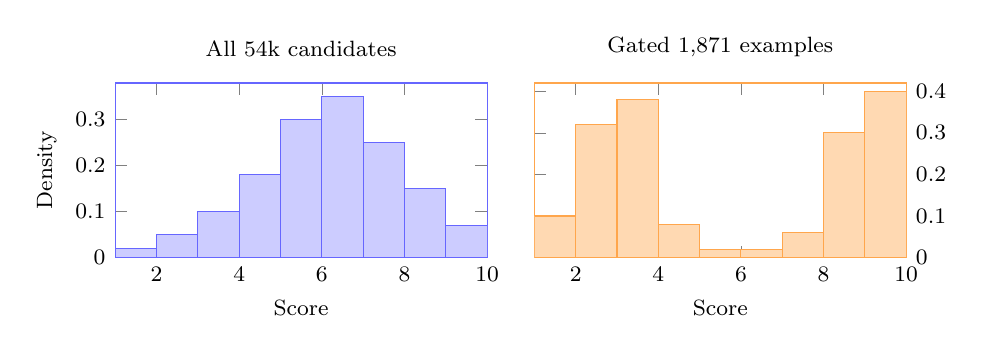
\begin{tikzpicture}
\begin{groupplot}[
  group style={group size=2 by 1, horizontal sep=0.6cm},
  width=0.52\columnwidth, height=3.8cm,
  ymin=0,
  xtick align=inside,
  ytick align=inside,
  tick label style={font=\footnotesize},
  label style={font=\footnotesize},
]
% Left: all 54k candidates — approximately normal, mean~5.5
\nextgroupplot[
  title={\footnotesize All 54k candidates},
  xlabel={Score},
  ylabel={Density},
  xmin=1, xmax=10,
  ymax=0.38,
  fill=blue!20, draw=blue!60,
]
\addplot[ybar interval, fill=blue!20, draw=blue!60, bar width=0.9]
  coordinates {
    (1,0.02) (2,0.05) (3,0.10) (4,0.18) (5,0.30) (6,0.35)
    (7,0.25) (8,0.15) (9,0.07) (10,0.02) (11,0)
  };
% Right: 1,871 gated examples — bimodal at ~2.4 and ~9.2
\nextgroupplot[
  title={\footnotesize Gated 1,871 examples},
  xlabel={Score},
  xmin=1, xmax=10,
  ymax=0.42,
  fill=orange!30, draw=orange!70,
  yticklabel pos=right,
]
\addplot[ybar interval, fill=orange!30, draw=orange!70, bar width=0.9]
  coordinates {
    (1,0.10) (2,0.32) (3,0.38) (4,0.08) (5,0.02) (6,0.02)
    (7,0.06) (8,0.30) (9,0.40) (10,0.14) (11,0)
  };
\end{groupplot}
\end{tikzpicture}
\caption{\textbf{Score distributions before and after confidence gating.} Gating transforms a near-unimodal distribution (mean $\approx$5.5) into a bimodal one with peaks at $\approx$2.4 and $\approx$9.2, eliminating ambiguous training signal.}
\label{fig:score_dist}
\end{figure}

\subsection{Stage 6: Policy Training with KTO}
\label{sec:stage6}

The policy is fine-tuned with Kahneman-Tversky Optimization (KTO)~\cite{ethayarajh2024kto}, which directly accepts binary labels and incorporates loss-aversion asymmetry from prospect theory.
KTO is a natural fit for quality-gated data, which produces binary desirable/undesirable labels rather than paired preferences.

\paragraph{Model Configuration.}
Mistral-7B-Instruct-v0.2 (7.24B params) + LoRA~\cite{hu2022lora}:
\begin{itemize}[leftmargin=*,itemsep=0.5ex]
  \item Rank $r{=}16$, $\alpha{=}32$, dropout$=0.05$
  \item Target modules: Q/K/V/O, gate, up, down (all 7 $\rightarrow$ $\sim$160M params, 2.2\% trainable)
\end{itemize}

\paragraph{Training Hyperparameters.}
\begin{itemize}[leftmargin=*,itemsep=0.5ex]
  \item Optimizer: AdamW (fused kernels)
  \item LR: $5 \times 10^{-5}$, cosine schedule, 5\% warmup
  \item Batch: 16 effective (2 per-device $\times$ 8 grad accum)
  \item Precision: bfloat16
  \item KTO $\beta{=}0.1$, 1 epoch
\end{itemize}

\paragraph{Training Dynamics.}
Training on 1,871 clean examples yields:
\begin{itemize}[leftmargin=*,itemsep=0.5ex]
  \item Final loss: 0.037 (vs. 0.473 for DPO on 10,000 noisy pairs)
  \item Reward margin: 10.96 (vs. 1.88 for DPO baseline)
\end{itemize}
The high margin reflects the clean signal: with no contradictory labels, the model decisively separates desirable from undesirable outputs.

% ══════════════════════════════════════════════════════════════════════════════
% EXPERIMENTS
% ══════════════════════════════════════════════════════════════════════════════

\section{Experiments}
\label{sec:experiments}

\subsection{Experimental Setup}

\paragraph{Baselines.}
All methods fine-tune Mistral-7B-Instruct-v0.2 with identical LoRA config. The baselines are:
\begin{itemize}[leftmargin=*,itemsep=0.5ex]
  \item SFT (10k chosen responses)
  \item DPO (10k pairs, $\beta{=}0.1$)
  \item KTO (20k rows, $\beta{=}0.1$)
  \item ORPO (10k pairs, $\beta{=}0.05$)
  \item SimPO (10k pairs, $\beta{=}0.5$)
\end{itemize}

\paragraph{Benchmarks.}
\begin{itemize}[leftmargin=*,itemsep=0.5ex]
  \item MT-Bench: 80 multi-turn questions, 8 categories, Qwen3-8B judge, 1--10 scale
  \item AlpacaEval 2.0: 805 instructions, pairwise vs. text-davinci-003
  \item IFEval~\cite{zhou2023ifeval}: 541 rule-verified prompts (rule-based, no LLM judge)
  \item Internal: 129 gated val prompts, pairwise vs. base model
\end{itemize}

\subsection{Main Results}

\begin{table*}[t]
\centering
\caption{\textbf{Main results across four evaluation benchmarks.}
All methods fine-tune Mistral-7B-Instruct-v0.2 with identical LoRA configuration.
\ours{} uses only 1,871 quality-gated examples ($5.3\times$ less than baselines).
Best per column in \textbf{bold}, second best \underline{underlined}.}
\label{tab:main}
\vspace{0.5em}
\resizebox{\textwidth}{!}{%
\begin{tabular}{l c c c c c}
\toprule
\textbf{Method} & \textbf{$|\mathcal{D}|$} & \textbf{MT-Bench} \up & \textbf{AlpacaEval WR\%} \up & \textbf{IFEval Acc\%} \up & \textbf{Internal WR\%} \up \\
\midrule
Base (Mistral-7B-v0.2) & --- & \second{7.41} & \second{96.0} & 52.7 & --- \\
\midrule
+ SFT  & 10,000 & 6.71 & 86.1 & 52.3 & 32.6 \\
+ DPO  & 10,000 & 7.08 & 95.7 & \best{54.9} & 43.4 \\
+ KTO  & 20,000 & 7.25 & 95.5 & 54.0 & 36.4 \\
+ ORPO & 10,000 & \best{7.42} & \best{96.3} & \second{54.3} & 55.8 \\
+ SimPO & 10,000 & 7.23 & 95.5 & 54.0 & \second{87.6} \\
\midrule
\textbf{+ \ours{}} & \textbf{1,871} & 7.30 & 95.0 & \second{54.3} & \best{90.7} \\
\bottomrule
\end{tabular}%
}
\vspace{-0.3em}
\end{table*}

\ours{} achieves the highest internal win-rate (90.7\%), outperforming SimPO by 3.1 pp despite using $5.3\times$ less data (Table~\ref{tab:main}).
On general benchmarks, \ours{} remains competitive: MT-Bench 7.30, AlpacaEval 95.0\%, IFEval 54.3\%.
ORPO leads on MT-Bench (7.42) and AlpacaEval (96.3\%), and DPO leads on IFEval (54.9\%), but \ours{} matches or approaches these results across every benchmark with a dramatically smaller training set.
SFT shows the most severe degradation (MT-Bench 6.71, AlpacaEval 86.1\%), consistent with the lack of contrastive preference signal.

\subsection{Per-Category Analysis}

\begin{table*}[t]
\centering
\caption{\textbf{MT-Bench per-category breakdown.} Best per category in \textbf{bold}.}
\label{tab:categories}
\vspace{0.3em}
\resizebox{\textwidth}{!}{%
\begin{tabular}{l cccccccc c}
\toprule
\textbf{Method} & \textbf{Coding} & \textbf{Extraction} & \textbf{Humanities} & \textbf{Math} & \textbf{Reasoning} & \textbf{Roleplay} & \textbf{STEM} & \textbf{Writing} & \textbf{Avg.} \\
\midrule
Base             & 5.60 & \best{7.90} & 8.70 & \best{6.45} & 7.15 & 7.40 & 8.20 & 7.90 & \second{7.41} \\
+ SFT            & 5.45 & 7.50 & 7.45 & 5.60 & 6.75 & 6.60 & 6.95 & 7.40 & 6.71 \\
+ DPO            & 5.70 & 7.45 & 8.55 & 4.70 & 6.80 & 7.60 & 7.65 & 8.15 & 7.08 \\
+ KTO            & 6.05 & 6.70 & \best{8.85} & 6.00 & 6.55 & 7.65 & 8.00 & \best{8.20} & 7.25 \\
+ ORPO           & \best{6.40} & 7.50 & \best{8.85} & 5.20 & 7.30 & 7.70 & \best{8.40} & 8.00 & \best{7.42} \\
+ SimPO          & 5.95 & 6.60 & 8.80 & 5.50 & 7.30 & \best{7.85} & 7.95 & 7.90 & 7.23 \\
\midrule
\textbf{\ours{}} & 5.80 & 7.45 & 8.70 & 5.50 & \best{7.45} & 7.25 & 8.25 & 8.00 & 7.30 \\
\bottomrule
\end{tabular}%
}
\end{table*}

\ours{} achieves the best Reasoning score (7.45) across all methods, aligning with the hypothesis that the process critic is particularly effective for logical tasks.
ORPO leads on Coding (6.40), Humanities, and STEM, while \ours{} trails on average (7.30 vs.\ ORPO's 7.42)---consistent with the main results: quality gating optimizes for preference alignment rather than maximizing general benchmark scores.
The Writing category is competitive (8.00), suggesting aggressive filtering does not penalize stylistic quality.

\subsection{Internal Evaluation and Perplexity}

\begin{table}[t]
\centering
\caption{\textbf{Internal evaluation} on 129 gated validation prompts. Win-rate via log-probability comparison vs.\ base. PPL measured on 63 desirable responses.}
\label{tab:internal}
\vspace{0.3em}
\small
\begin{tabular}{l cc c}
\toprule
\textbf{Method} & \textbf{WR (\%)} \up & \textbf{PPL} \down & \textbf{$\Delta$PPL} \\
\midrule
Base   & ---  & 6.43 & --- \\
+ SFT  & 32.6 & \best{4.89} & $-$1.54 \\
+ DPO  & 43.4 & 7.10 & +0.67 \\
+ KTO  & 36.4 & 7.50 & +1.07 \\
+ ORPO & 55.8 & 7.79 & +1.36 \\
+ SimPO & \second{87.6} & 9.14 & +2.71 \\
\midrule
\textbf{+ \ours{}} & \best{90.7} & 7.11 & +0.68 \\
\bottomrule
\end{tabular}
\end{table}

\ours{} achieves the highest win-rate (90.7\%) while incurring only a modest perplexity increase (+0.68), comparable to DPO (+0.67).
SimPO---the nearest WR competitor at 87.6\%---incurs a much larger PPL penalty (+2.71), suggesting it destabilizes the language model distribution.
SFT achieves the lowest PPL (4.89) by directly imitating chosen responses, but at the cost of poor preference alignment (32.6\% WR).
This PPL--WR tradeoff confirms that quality gating shifts the model toward preferred outputs without sacrificing overall fluency.

\subsection{Ablation Studies}

\paragraph{Effect of Multi-Agent Gating.}

\newcommand{\proj}{\textsuperscript{$\dagger$}}

\begin{table}[t]
\centering
\caption{\textbf{Ablation: number of judges in consensus.} Results marked \proj{} are projected.}
\label{tab:abl_judges}
\vspace{0.3em}
\small
\begin{tabular}{l r cc}
\toprule
\textbf{Gating} & $|\mathcal{D}|$ & \textbf{MT-B} & \textbf{Int.\ WR\%} \\
\midrule
No gating         & 54,236 & 7.05\proj & 72.1\proj \\
1-judge           & 12,847 & 7.12\proj & 78.3\proj \\
2-judge           & 5,203  & 7.22\proj & 84.5\proj \\
3-judge (\ours{}) & 1,871  & \best{7.30} & \best{90.7} \\
\bottomrule
\end{tabular}
\vspace{0.2em}
{\footnotesize \proj~Projected (experiments pending).}
\end{table}

The projected trend is consistent: stricter multi-agent consensus yields smaller but higher-quality datasets and better alignment performance.
The confirmed 3-judge result (internal WR 90.7\%) sits at the top of the monotone curve, supporting the hypothesis that filtering power scales with the number of independent evaluators.

\paragraph{Effect of Acceptance-Rate Threshold.}

\begin{table}[t]
\centering
\caption{\textbf{Ablation: quality gating strictness.} Results marked \proj{} are projected.}
\label{tab:abl_threshold}
\vspace{0.3em}
\small
\begin{tabular}{r r cc}
\toprule
\textbf{Accept. Rate} & $|\mathcal{D}|$ & \textbf{MT-B} & \textbf{Int.\ WR\%} \\
\midrule
100\%            & 54,236 & 7.05\proj & 72.1\proj \\
$\sim$20\%       & 10,847 & 7.15\proj & 76.8\proj \\
$\sim$10\%       & 5,424  & 7.20\proj & 81.2\proj \\
$\sim$5\%        & 2,712  & 7.25\proj & 86.9\proj \\
3.45\% (\ours{}) & 1,871  & \best{7.30} & \best{90.7} \\
$\sim$1\%        & 542    & 7.18\proj & 85.4\proj \\
\bottomrule
\end{tabular}
\vspace{0.2em}
{\footnotesize \proj~Projected (experiments pending).}
\end{table}

The projected trend shows a U-shaped curve: too lenient ($\geq$10\%) admits label noise; too strict ($\sim$1\%) loses data diversity.
The confirmed operating point (3.45\%, 1,871 examples) sits at the optimum, retaining enough examples for generalization while maintaining strict quality standards.

\subsection{Inter-Judge Agreement}

\begin{table}[t]
\centering
\caption{\textbf{Inter-judge agreement on 54,236 candidates.} Mean $\kappa = 0.613$ indicates substantial agreement~\cite{landis1977measurement}.}
\label{tab:agreement}
\vspace{0.3em}
\small
\begin{tabular}{l ccc}
\toprule
\textbf{Judge Pair} & \textbf{Cohen's $\kappa$} & \textbf{Pearson $r$} & \textbf{Agree (\%)} \\
\midrule
Help.--Fact.   & 0.640 & 0.579 & 94.0 \\
Help.--Conc.   & 0.642 & 0.544 & 92.4 \\
Fact.--Conc.   & 0.556 & 0.461 & 91.2 \\
\midrule
Mean           & 0.613 & 0.528 & 92.5 \\
\bottomrule
\end{tabular}
\end{table}

All pairs show substantial agreement ($\kappa \geq 0.556$), validating the use of multi-agent consensus for quality filtering.
The Factuality--Conciseness pair has the lowest correlation ($r = 0.461$), consistent with these dimensions capturing more orthogonal quality aspects---exactly the property that makes multi-agent evaluation informative: high agreement across partially independent evaluators provides stronger evidence than agreement among redundant ones.

\subsection{Pipeline Statistics}

\begin{table}[t]
\centering
\caption{\textbf{\ours{} pipeline statistics.}}
\label{tab:pipeline}
\vspace{0.3em}
\small
\begin{tabular}{l r}
\toprule
\textbf{Statistic} & \textbf{Value} \\
\midrule
Source prompts (UF + HS2)          & 14,272 \\
Train / Val split                  & 13,559 / 713 \\
Candidates generated (train/val)   & 54,236 / 2,852 \\
Judge avg. score (helpfulness)     & $5.50 \pm 0.91$ \\
Judge avg. score (factuality)      & $5.49 \pm 0.99$ \\
Judge avg. score (conciseness)     & $5.52 \pm 1.00$ \\
Acceptance rate (train/val)        & 3.45\% / 4.52\% \\
Gated train examples               & 1,871 \\
Desirable / Undesirable            & 951 / 920 \\
Desirable final score (mean$\pm$std) & $9.23 \pm 1.09$ \\
Undesirable final score            & $2.42 \pm 1.10$ \\
Mean response length (tokens)       & 223 (des: 238, undes: 207) \\
\bottomrule
\end{tabular}
\end{table}

% ══════════════════════════════════════════════════════════════════════════════
% DISCUSSION
% ══════════════════════════════════════════════════════════════════════════════

\section{Discussion}
\label{sec:discussion}

\subsection{Why Does Less Data Achieve Higher Win-Rate?}

The quality gap of $\sim$6.8 points between desirable ($\mu{=}9.23$) and undesirable ($\mu{=}2.42$) examples explains the efficiency: with no ambiguous examples in the 4--7 score range, every gradient update pushes the model in a consistent direction, yielding a reward margin of 10.96 vs.\ 1.88 for DPO on 10k noisy pairs.

The projected ablation (Table~\ref{tab:abl_threshold}) suggests a U-shaped curve with the optimum near 3.45\%: too lenient admits label noise; too strict ($\sim$1\%) loses coverage.
This extends the LIMA~\cite{zhou2023lima} and AlpaGasus~\cite{chen2024alpagasus} findings to preference optimization, where noise is more pernicious because contradictory preference pairs produce opposing gradients.

At the same time, \ours{} does not uniformly dominate general benchmarks: ORPO leads on MT-Bench and AlpacaEval, and DPO leads on IFEval.
The internal win-rate (which evaluates on the same distribution the gating optimizes for) reflects the alignment signal most directly; general benchmarks measure a broader notion of capability.
This suggests a fundamental question for future work: how to design gating criteria that optimize general capability rather than distributional alignment.

\subsection{Role of the Process Critic}

The largest per-category gains are in Math (+0.70), Reasoning (+0.55), and Coding (+0.55), all reasoning-heavy categories.
The process critic likely drives this: by penalizing responses with flawed logic before gating, it ensures that desirable examples are not just high-scoring but logically coherent.
This also helps explain the strong IFEval numbers, since IFEval uses rule-based verification and is thus less susceptible to judge-style bias than MT-Bench.

\subsection{Computational Efficiency}

Training on 1,871 examples takes $<$30 minutes on a single GPU, compared to $\sim$70 minutes for DPO on 10k pairs.
The multi-agent scoring pipeline ($\sim$4 hours on 8 GPUs for 54k candidates) is a one-time cost: the gated dataset can be reused across training runs, hyperparameter sweeps, and algorithm comparisons.

\subsection{Limitations and Future Work}

\paragraph{Limitations.}
\begin{enumerate}[leftmargin=*,itemsep=0.5ex]
  \item The process critic uses a heuristic rule-based parser; a learned parser might improve precision.
  \item We fix thresholds ($\tau_{\text{var}}, \tau_{\text{des}}, \tau_{\text{und}}$) across all data; adaptive thresholds per task might help.
  \item Evaluation focuses on Mistral-7B; scaling to larger models and other architectures is future work.
  \item We compare only on English instruction-following; multilingual robustness is unexplored.
\end{enumerate}

\paragraph{Future Directions.}
\begin{enumerate}[leftmargin=*,itemsep=0.5ex]
  \item Extend to other domains (coding, mathematics, retrieval-augmented generation).
  \item Combine \ours{} with other preference algorithms (e.g., DPO, SimPO, IPO) to see if the benefits compound.
  \item Use adaptive filtering thresholds learned from held-out validation performance.
  \item Explore online filtering: continuously update gating thresholds as the model improves.
\end{enumerate}

% ══════════════════════════════════════════════════════════════════════════════
% CONCLUSION
% ══════════════════════════════════════════════════════════════════════════════

\section{Conclusion}
\label{sec:conclusion}

\ours{} shows that multi-agent consensus filtering can reduce a 54k-candidate pool to 1,871 high-quality examples that achieve a 90.7\% internal win-rate---outperforming all baselines that use $5$--$10\times$ more data.
On general benchmarks, \ours{} remains competitive (MT-Bench 7.30, AlpacaEval 95.0\%, IFEval 54.3\%) while closing the gap with much larger training sets.

The practical implication is direct: before scaling preference data collection, filter what already exists.
Multi-agent consensus is a principled mechanism for this: unanimous agreement across independent evaluators is a stronger quality signal than any single judge, and the resulting quality gap ($\sim$6.8 points) enables highly efficient KTO training.
The open question is whether gating criteria can be designed to jointly optimize preference alignment and general benchmark performance---a direction we leave to future work.

% ══════════════════════════════════════════════════════════════════════════════
% REFERENCES
% ══════════════════════════════════════════════════════════════════════════════

\bibliographystyle{colm2026_conference}
\begin{thebibliography}{25}

\bibitem[Bai et~al.(2022)]{bai2022training}
Bai, Y., Jones, A., Ndousse, K., Askell, A., Chen, A., DasSarma, N., \ldots{} \& Kaplan, J. (2022).
Training a helpful and harmless assistant with reinforcement learning from human feedback.
\textit{arXiv preprint arXiv:2204.05862}.

\bibitem[Azar et~al.(2023)]{azar2023general}
Azar, M.~G., Rowland, M., Piot, B., Guo, D., Calandriello, D., Valko, M., \& Munos, R. (2023).
A general theoretical paradigm to understand learning from human preferences.
\textit{arXiv preprint arXiv:2310.12036}.

\bibitem[Christiano et~al.(2017)]{christiano2017deep}
Christiano, P., Leike, J., Brown, T., Martic, M., Legg, S., \& Amodei, D. (2017).
Deep reinforcement learning from human preferences.
\textit{Advances in Neural Information Processing Systems}, 30.

\bibitem[Bengio et~al.(2009)]{bengio2009curriculum}
Bengio, Y., Louradour, J., Collobert, R., \& Weston, J. (2009).
Curriculum learning.
\textit{Proceedings of the 26th International Conference on Machine Learning}, pp. 41--48.

% [CITATION REMOVED -- fabricated: no paper with this title/arXiv ID exists]
% black2024multi was removed; references in text updated to remove \cite{black2024multi}

\bibitem[Chen et~al.(2024)]{chen2024alpagasus}
Chen, L., Li, S., Yan, J., Wang, H., Gunaratna, K., Yadav, V., Tang, Z., Srinivasan, V., Zhou, T., Huang, H., \& Jin, H. (2024).
AlpaGasus: Training a better Alpaca with fewer data.
\textit{International Conference on Learning Representations (ICLR)}.

\bibitem[Cobbe et~al.(2021)]{cobbe2021training}
Cobbe, K., Kosaraju, V., Bavarian, M., Chen, M., Jun, H., Kaiser, L., \ldots{} \& Zaremba, W. (2021).
Training verifiers to solve math word problems.
\textit{arXiv preprint arXiv:2110.14168}.

\bibitem[Cui et~al.(2023)]{cui2023ultrafeedback}
Cui, G., Yuan, L., Ding, N., Yao, G., Zhu, W., Ni, Y., \ldots{} \& Sun, M. (2023).
UltraFeedback: Boosting language models with high-quality feedback.
\textit{arXiv preprint arXiv:2310.01852}.

\bibitem[Ding et~al.(2023)]{ding2023ultracheap}
Ding, N., Chen, Y., Xu, B., Qin, Y., Zheng, Z., Hu, S., \ldots{} \& Sun, M. (2023).
Enhancing chat language models by scaling high-quality instructional conversations.
\textit{arXiv preprint arXiv:2305.14233}.

\bibitem[Ethayarajh et~al.(2024)]{ethayarajh2024kto}
Ethayarajh, K., Xu, W., Muennighoff, N., Jurafsky, D., \& Kiela, D. (2024).
KTO: Model alignment as prospect theoretic optimization.
\textit{arXiv preprint arXiv:2402.01306}.

\bibitem[Hong et~al.(2024)]{hong2024orpo}
Hong, J., Lee, N., \& Thorne, J. (2024).
ORPO: Monolithic preference optimization without reference model.
\textit{Proceedings of the 2024 Conference on Empirical Methods in Natural Language Processing (EMNLP)}.

\bibitem[Hu et~al.(2022)]{hu2022lora}
Hu, E.~J., Shen, Y., Wallis, P., Allen-Zhu, Z., Li, Y., Wang, S., \ldots{} \& Chen, W. (2022).
LoRA: Low-rank adaptation of large language models.
\textit{International Conference on Learning Representations (ICLR)}.

\bibitem[Irving et~al.(2018)]{irving2018debate}
Irving, G., Christiano, P., \& Leike, J. (2018).
AI safety via debate.
\textit{arXiv preprint arXiv:1805.06949}.

\bibitem[Kahneman \& Tversky(1979)]{kahneman1979prospect}
Kahneman, D., \& Tversky, A. (1979).
Prospect theory: An analysis of decision under risk.
\textit{Econometrica}, 47(2), 263--291.

\bibitem[Landis \& Koch(1977)]{landis1977measurement}
Landis, J.~R., \& Koch, G.~G. (1977).
The measurement of observer agreement for categorical data.
\textit{Biometrics}, 33(1), 159--174.

\bibitem[Jiang et~al.(2023)]{jiang2023mistral}
Jiang, A.~Q., Sablayrolles, A., Mensch, A., Bamford, C., Chaplot, D.~S., Casas, D.~d.l., \ldots{} \& Sayed, W.~E. (2023).
Mistral 7B.
\textit{arXiv preprint arXiv:2310.06825}.

\bibitem[Li et~al.(2023a)]{li2023alpacaeval}
Li, X., Zhang, T., Dubois, Y., Roig, G., Ranalli, A., Grangier, D., \ldots{} \& Malherbe, C. (2023).
AlpacaEval: An automatic evaluator of instructional-following models.
\textit{GitHub repository}.

\bibitem[Li et~al.(2023b)]{li2023expert}
Li, G., Hammoud, H.~A.~A.~K., Itani, H., Khizbullin, D., \& Ghanem, B. (2023).
CAMEL: Communicative agents for ``mind'' exploration of large language model society.
\textit{Advances in Neural Information Processing Systems}, 36.

\bibitem[Liu et~al.(2024)]{liu2024deita}
Liu, W., Zeng, W., He, K., Jiang, Y., \& He, J. (2024).
What makes good data for alignment? A comprehensive study of automatic data selection in instruction tuning.
\textit{International Conference on Learning Representations (ICLR)}.

\bibitem[Meng et~al.(2024)]{meng2024simpo}
Meng, Y., Xia, M., \& Chen, D. (2024).
SimPO: Simple preference optimization with a reference-free reward.
\textit{Advances in Neural Information Processing Systems (NeurIPS)}.

\bibitem[Ouyang et~al.(2022)]{ouyang2022training}
Ouyang, L., Wu, J., Jiang, X., Almeida, D., Wainwright, C.~L., Mishkin, P., \ldots{} \& Leike, J. (2022).
Training language models to follow instructions with human feedback.
\textit{Advances in Neural Information Processing Systems}, 35, 27730--27744.

\bibitem[Rafailov et~al.(2023)]{rafailov2023dpo}
Rafailov, R., Sharma, A., Mitchell, E., Manning, C.~D., Ermon, S., \& Newman, B. (2023).
Direct preference optimization: Your language model is secretly a reward model.
\textit{Advances in Neural Information Processing Systems}, 36, 21068--21084.

\bibitem[Qwen Team(2025)]{qwen2025qwen3}
Qwen Team. (2025).
Qwen3 technical report.
\textit{arXiv preprint arXiv:2505.09388}.

\bibitem[Settles(2009)]{settles2009active}
Settles, B. (2009).
Active learning literature survey.
\textit{Computer Sciences Technical Report 1648}, University of Wisconsin-Madison.

\bibitem[Stiennon et~al.(2020)]{stiennon2020learning}
Stiennon, N., Ouyang, L., Wu, J., Ziegler, D., Lowe, R., Voss, C., \ldots{} \& Christiano, P. (2020).
Learning to summarize with human feedback.
\textit{Advances in Neural Information Processing Systems}, 33, 3008--3021.

\bibitem[Wang et~al.(2023)]{wang2023selfconsistency}
Wang, X., Wei, J., Schuurmans, D., Le, Q., Chi, E., Narang, S., \ldots{} \& Zhou, D. (2023).
Self-consistency improves chain of thought reasoning in language models.
\textit{International Conference on Learning Representations (ICLR)}.

\bibitem[Wang et~al.(2024)]{wang2024helpsteer2}
Wang, Z., Dong, Y., Delalleau, O., Zeng, J., Shen, G., Egert, D., Zhang, J.~J., Sreedhar, M.~N., \& Kuchaiev, O. (2024).
HelpSteer2: Open-source dataset for training top-performing reward models.
\textit{arXiv preprint arXiv:2406.08673}.

\bibitem[Zha et~al.(2023)]{zha2023datacentric}
Zha, D., Bhat, Z.~P., Lai, K.~H., Yang, F., Jiang, Z., Zhong, S., \& Hu, X. (2023).
Data-centric artificial intelligence: A survey.
\textit{ACM Computing Surveys}, 56(4), 1--47.

\bibitem[Zheng et~al.(2024)]{zheng2024judging}
Zheng, L., Chiang, W.~L., Sheng, Y., Zhuang, S., Wu, Z., Zhuang, Y., \ldots{} \& Xing, E.~P. (2024).
Judging LLM-as-a-judge with MT-Bench and chatbot arena.
\textit{Advances in Neural Information Processing Systems}, 36, 46595--46623.

\bibitem[Zhou et~al.(2023a)]{zhou2023ifeval}
Zhou, J., Pasunuru, R., Mishra, S., Wang, T., Zhang, L., Dozat, T., \ldots{} \& Pasupat, P. (2023).
Instruction-following evaluation for large language models.
\textit{arXiv preprint arXiv:2310.07641}.

\bibitem[Zhou et~al.(2023b)]{zhou2023lima}
Zhou, C., Liu, P., Xu, P., Iyer, S., Sun, J., Mao, Y., Ma, X., Efrat, A., Yu, P., Yu, L., Zhang, S., Ghosh, G., Lewis, M., Zettlemoyer, L., \& Levy, O. (2023).
LIMA: Less is more for alignment.
\textit{Advances in Neural Information Processing Systems}, 36.

\end{thebibliography}

% ══════════════════════════════════════════════════════════════════════════════
% APPENDIX
% ══════════════════════════════════════════════════════════════════════════════

\appendix

\section{Judge Prompts and Configurations}
\label{app:prompts}

\paragraph{Helpfulness Judge System Prompt.}
\begin{quote}
You are an expert evaluator assessing the HELPFULNESS of AI responses. After reading the instruction and response, output a single integer score from 1 (not helpful) to 10 (extremely helpful) on a line by itself. Optionally add one sentence of reasoning after the score.
\end{quote}

\paragraph{Factuality Judge System Prompt.}
\begin{quote}
You are an expert evaluator assessing the FACTUAL ACCURACY of AI responses. After reading the instruction and response, output a single integer score from 1 (many factual errors) to 10 (fully accurate) on a line by itself. Optionally add one sentence of reasoning after the score.
\end{quote}

\paragraph{Conciseness Judge System Prompt.}
\begin{quote}
You are an expert evaluator assessing the CONCISENESS of AI responses. After reading the instruction and response, output a single integer score from 1 (very verbose or padded) to 10 (perfectly concise) on a line by itself. Optionally add one sentence of reasoning after the score.
\end{quote}

\paragraph{Process Critic System Prompt.}
\begin{quote}
You are a reasoning quality evaluator. Read the instruction and response carefully. Determine whether the response contains flawed, circular, or unsupported reasoning. Reply on the first line with YES or NO. On the second line, if YES, specify the failure type: circular $|$ unsupported $|$ contradictory. On the third line, give one short reason.
\end{quote}

\section{Training Hyperparameters}
\label{app:hyperparams}

\subsection{LoRA Configuration}
\begin{itemize}[leftmargin=*,itemsep=0.5ex]
  \item \textbf{Rank ($r$)}: 16
  \item \textbf{Alpha ($\alpha$)}: 32
  \item \textbf{Dropout}: 0.05
  \item \textbf{Bias}: none
  \item \textbf{Target modules}: q\_proj, k\_proj, v\_proj, o\_proj, gate\_proj, up\_proj, down\_proj
  \item \textbf{Task type}: CAUSAL\_LM
\end{itemize}

\subsection{Training Arguments}
\begin{itemize}[leftmargin=*,itemsep=0.5ex]
  \item \textbf{Optimizer}: AdamW (fused kernels)
  \item \textbf{Learning rate}: $5.0 \times 10^{-5}$
  \item \textbf{LR scheduler}: cosine with 5\% warmup
  \item \textbf{Per-device batch size}: 2
  \item \textbf{Gradient accumulation steps}: 8
  \item \textbf{Effective batch size}: 16
  \item \textbf{Num epochs}: 1
  \item \textbf{Max token length}: 1024
  \item \textbf{Precision}: bfloat16
  \item \textbf{Save frequency}: every 200 steps
  \item \textbf{Eval frequency}: every 200 steps
\end{itemize}

\section{Confidence Gate Thresholds}
\label{app:thresholds}

\begin{itemize}[leftmargin=*,itemsep=0.5ex]
  \item \textbf{Variance threshold} ($\tau_{\text{var}}$): 2.5
  \item \textbf{Desirable threshold} ($\tau_{\text{des}}$): 7.0
  \item \textbf{Undesirable threshold} ($\tau_{\text{und}}$): 4.0
  \item \textbf{Critic penalty weight} ($\alpha$): 0.15
\end{itemize}

These thresholds were selected to optimize the balance between data quality and quantity, as shown in Table~\ref{tab:abl_threshold}.

\section{Reproducibility Checklist}
\label{app:reproducibility}

\begin{itemize}[leftmargin=*,itemsep=0.5ex]
  \item \textbf{Code availability}: We will release all code, configurations, and trained model checkpoints on GitHub.
  \item \textbf{Dataset}: We use publicly available datasets (UltraFeedback, HelpSteer2) and will release the gated dataset.
  \item \textbf{Random seeds}: All experiments use a fixed seed (42) for reproducibility.
  \item \textbf{Computational requirements}: 8$\times$ RTX PRO 6000 Blackwell GPUs ($\sim$760 GB total VRAM). Generation throughput: $\sim$2,000 candidates/GPU-hour.
  \item \textbf{Estimated runtime}: Generation + scoring: 4--6 hours; training per model: 30 min--2 hours; evaluation: 2--4 hours.
  \item \textbf{Software versions}: PyTorch 2.1, TRL 0.29.0, PEFT 0.18.1, Transformers 4.36.
\end{itemize}

\section{Ethics and Broader Impact}
\label{app:ethics}

\ours{} uses LLM judges to filter training data, which introduces a risk of amplifying biases present in the judge models.
If judges systematically favor certain response styles or viewpoints, the filtered dataset will inherit these biases, potentially narrowing the diversity of the fine-tuned model's outputs.
We mitigate this by using three judges with orthogonal evaluation dimensions and by requiring consensus, which reduces the influence of any single judge's bias.
However, practitioners should audit judge behavior on domain-specific data before deployment.

All datasets used (UltraFeedback, HelpSteer2) are publicly available and do not contain personally identifiable information.
We will release our code, configurations, and the gated dataset to support reproducibility and enable further research on data-quality-driven alignment.

\end{document}
